\setcounter{page}{1}
\chapter{INTRODU\c{C}\~AO}  %%Nesta linha, dentro de { }, digita-se em CAIXA ALTA, como apresentado aqui
\label{chap:01}
A engenharia de \textit{software} surgiu como um esforço de aplicar processos que pudessem dar maior assertividade nos projetos de \textit{software}. Através desses esforços surgiram vários modelos que contribuíram para melhorar o cenário de desenvolvimento. Pode-se dizer que esses esforços foram também impulsionados através do mercado, o qual se torna cada vez mais competitivo e exige que os projetos de \textit{software} tenham que ser desenvolvidos com extrema qualidade e de forma rápida, repetida e confiável.
Dentre as várias metodologias que surgiram, uma metodologia está ganhando bastante destaque no mercado atual: o \textit{lean}. \citeonline{4222727} aponta que iniciativas \textit{lean} (ou enxuta)\footnote{Neste trabalho é empregado a palavra em inglês lean.}  tem sido utilizadas com sucesso em vários setores como manufatura, logística, serviços e no desenvolvimento de produtos, a fim de garantir uma melhor entrega no que tange ao custo, qualidade e prazo. Uma pergunta que surge naturalmente é: “É possível aplicar os mesmos conceitos já aplicados em outros setores para o \textit{software} ?”. Esse trabalho propõe-se a responder essa e outras perguntas sobre aplicação do \textit{lean} no contexto de \textit{software}. 
Na seção seguinte, é mostrado alguns trabalhos na linha de pesquisa do \textit{lean} e que contribuíram para o trabalho.

\section{TRABALHOS RELACIONADOS}

No trabalho  de \citeonline{4222727} é mostrado um breve tutorial para aplicação de \textit{lean} no desenvolvimento de \textit{software}. O \textit{lean} é focado em sete princípios:

\begin{itemize}
	\item Eliminar desperdício;
	\item Incorporar qualidade;
	\item	Criar conhecimento;
	\item	Adiar compromisso;
	\item	Entregar rápido;
	\item	Respeitar pessoas e
	\item	Otimizar o todo.
\end{itemize}


Todo esse grupo de princípios, segundo esse trabalho, fornece uma orientação de como entregar um \textit{software} de forma rápida, melhor e com um custo menor. Neste trabalho é afirmado que o desenvolvimento de software lean fornece a teoria por trás das práticas utilizadas pelo desenvolvimento ágil. Além disso, o \textit{lean} fornece para as empresas uma série de princípios para melhorar o processo de engenharia de software com a finalidade de trazer melhora no contexto do cliente, domínio do negócio, capacidade de desenvolvimento e em uma eventual situação única que a empresa enfrente.

Neste trabalho um tutorial foi feito com uma turma e a aplicabilidade do \textit{lean}\textit{ no} desenvolvimento de \textit{software} é feita através dos princípios fundamentais do \textit{lean}\textit{.} No princípio do desperdício, além de sua explicação no contexto de \textit{lean}\textit{,} foi mostrado como enxergar o desperdício no contexto do desenvolvimento e explanado os sete desperdícios no desenvolvimento de \textit{software}. Nesta etapa, a classe foi divida em grupos de até sete pessoas e foi feito um mapeamento de fluxo de valor da experiência de alguém no grupo. Após a elaboração, os grupos apresentaram seu mapa e receberam críticas dos outros participantes.

Para o próximo conceito do \textit{lean}\textit{,} qualidade, foram apresentados conceitos como: TDD (test-driven development), teste unitário automatizado e teste de aceitação. Essa etapa não focou muito em como fazer, mas o porquê da importância dessas práticas para o \textit{lean}\textit{.}

Uma análise racional, no que se refere ao conhecimento, foi feita sobre a questão de postergar os compromissos (princípio do pensamento \textit{lean}). Também foram apresentados métodos que visam preservar o conhecimento de forma que os times não tenham que reaprender o que já foi aprendido. Além disso, foi feita uma discussão dos benefícios da utilização de uma abordagem que envolve explorar múltiplas soluções em vez de focar em apenas uma.

Na questão de velocidade, é discutido a aplicação da teoria das filas no desenvolvimento de \textit{\textit{}.} Nela foi mostrado o porquê de longas filas serem prejudiciais ao desenvolvimento e também foi mostrado como evita-las. Além disso, é mostrado que ciclos de vida rápidos tendem a dar uma qualidade maior ao projeto de \textit{software} e reduzir seu custo.

Por fim, foi discutido a importância de enxergar um sistema como um todo. Através dessa discussão foi explanado que não é suficiente focar apenas no desenvolvimento em si, assim foi mostrado como mudar o foco do desenvolvimento para os esforços dos  objetivos em geral, ou seja, o produto ou o processo apoiado pelo \textit{software}. 

No trabalho de \citeonline{7107412}, a abordagem de migração para o \textit{lean} de uma empresa de \textit{software} também foi feita a partir da medição do fluxo de valor da organização com posterior utilização desses dados para migração. Essa equipe já utilizava a metodologia ágil de desenvolvimento. Para medir o fluxo de valor é medido aspectos de interesse das atividades, recursos utilizados e artefatos produzidos. É importante notar que, como assinala Janes (2015), o que é de interesse do ponto de vista para os objetivos de uma empresa não necessariamente é para outra. Por isso é utilizado a abordagem GQM+. Essa abordagem foi necessária a fim de ajudar na correspondência das estratégias com a necessidade de informação e das medidas. Os dados obtidos são usados para entender melhor o processo de desenvolvimento de \textit{software}. Uma técnica chamada Andon é então utilizada no sentido de fornecer um mecanismo para visualização dos dados por qualquer pessoa com o menor esforço possível. Através desse mecanismo de visualização, um feedback para o time  é feito no sentido de guia-los nos seus objetivos. Na Figura \ref{fig:01} é mostrado um mapa que ilustra a dinâmica do \textit{lean} em uma empresa que emprega o processo de desenvolvimento ágil. 

\begin{figure}
\begin{center}
\caption{Mapas de conceito descrevendo os blocos de construção do desenvolvimento de software lean}
\label{fig:01}
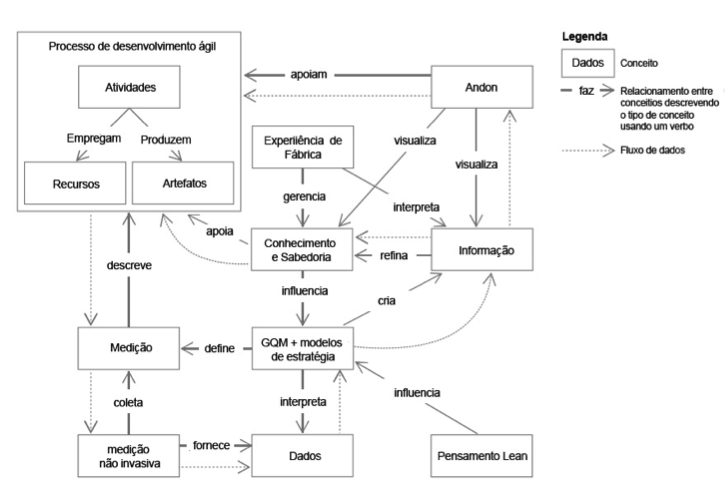
\includegraphics[width=13cm]{assets/figura1} \\
\fonte{Adaptado de \cite{7107412}.}
\end{center}
\end{figure}


